\documentclass[conference]{IEEEtran}
\IEEEoverridecommandlockouts

\usepackage{cite}
\usepackage{amsmath,amssymb,amsfonts}
\usepackage{algorithmic}
\usepackage{graphicx}
\usepackage{textcomp}
\usepackage{xcolor}
\usepackage{booktabs}
\usepackage{array}
\usepackage{placeins}

\graphicspath{{figures/}}

\def\BibTeX{{\rm B\kern-.05em{\sc i\kern-.025em b}\kern-.08em
    T\kern-.1667em\lower.7ex\hbox{E}\kern-.125emX}}

\begin{document}

\title{Geometric Segmentation of Steppable Surfaces in Simulated LiDAR
Staircase Point Clouds: A Comparative Evaluation for Stair-Climbing Robot
Perception}

\author{\IEEEauthorblockN{Samar Gamil Ahmed Aqaln Aldubai}
\IEEEauthorblockA{\textit{Dept. of Information and Computer Engineering} \\
\textit{Politeknik Elektronika Negeri Surabaya (PENS)}\\
Surabaya, Indonesia \\
\texttt{samar@pasca.student.pens.ac.id}}
}

\maketitle

\begin{abstract}
Walking upstairs with legged and tracked robots requires the ability to reliably
perceive where a foot could be safely placed. We cast this as a point-cloud
segmentation problem where each point of a staircase must be tagged as a
\emph{steppable} tread, a vertical \emph{riser}, or \emph{other} (edges, noise,
outliers). We create a parametric generator which analytically synthesizes a
4-step staircase, with forced Gaussian surface jitter, isotropic LiDAR noise, and
uniform outliers, producing a fully labeled cloud of $\sim$18k points. We implement
and analyze four conventional, non-learning geometric algorithms on this data:
(i) per-point PCA normal analysis, (ii) multi-plane RANSAC, (iii) normal-augmented
DBSCAN with per-cluster slope classification, and (iv) height-histogram tread
identification. We report Accuracy, Precision, Recall, F1 and IoU for the steppable
class, and assess robustness to sensor noise and outliers. The PCA-normal technique
yields greatest overall agreement (F1~$=0.913$, IoU~$=0.840$), whereas DBSCAN and
height-histogram provide the highest steppable precision ($\approx0.98$), which is
the metric most directly controlling foothold safety. We propose that a
precision-oriented operating point is preferable for a stair-following robot and
examine the consequences of the observed noise sensitivity.
\end{abstract}

\begin{IEEEkeywords}
point cloud, segmentation, RANSAC, DBSCAN, surface normals, LiDAR, stair-climbing
robot, geometric perception
\end{IEEEkeywords}

\section{Introduction}
\IEEEPARstart{W}{alking} up stairs is a classic problem for mobile robots
functioning in human contexts. Before any motion planning, the robot has to
transform a raw range scan into a semantic understanding of the geometry,
especially \emph{which surfaces can bear a foot}~\cite{kanoulas2018footstep}. A
tread misclassified as a riser just wastes a candidate foothold, whereas a riser
or an edge misclassified as a tread can cause a misstep. Steppable-surface
segmentation is asymmetric and safety-critical, i.e., false positives are
considerably more expensive than false negatives.

This work gives a systematic, reproducible examination of traditional geometric
segmentation for this problem. Point-cloud segmentation has been widely
studied~\cite{nguyen2013segmentation}, and learning-based segmenters such as
PointNet~\cite{qi2017pointnet} now dominate large-scale benchmarks. However, they
need labelled training data and offer limited interpretability. Instead of learning
from data, we leverage the strong geometric priors of a staircase (big planar
horizontal treads, large vertical risers, thin clutter at their connections) and
compare four algorithms that encapsulate these priors in different ways. Our work
contributes:
\begin{itemize}
\item a parametric generator that generates a 4-step staircase point cloud from
explicit equations, with realistic LiDAR noise, outliers and exact ground-truth
labels;
\item an implementation and head-to-head comparison of four geometric methods
(PCA normals, multi-plane RANSAC, normal-augmented DBSCAN, height-histogram);
\item a noise- and outlier-sensitivity study of the steppable-class metrics; and
\item a precision-oriented safety analysis for foothold selection by a
stair-following robot.
\end{itemize}

\section{Staircase Point-Cloud Generation}
\label{sec:data}
We construct a staircase with $N_s=4$ steps of width $w$ (x-axis), tread depth $d$
(y-axis) and step height $h$ (z-axis). For each step $i\in\{0,\dots,N_s-1\}$ the two
dominant surfaces are sampled as follows.

\textbf{Tread (steppable, horizontal):}
\begin{equation}
\begin{cases}
x \sim \mathcal{U}(0, w) \\
y \sim \mathcal{U}(i\,d,\; (i{+}1)\,d) \\
z = i\,h + \epsilon_z, \quad \epsilon_z \sim \mathcal{N}(0, \sigma_z^2)
\end{cases}
\label{eq:tread}
\end{equation}

\textbf{Riser (vertical):}
\begin{equation}
\begin{cases}
x \sim \mathcal{U}(0, w) \\
y = i\,d + \epsilon_y, \quad \epsilon_y \sim \mathcal{N}(0, \sigma_y^2) \\
z \sim \mathcal{U}\big((i{-}1)\,h,\; i\,h\big)
\end{cases}
\label{eq:riser}
\end{equation}

We utilize $w=2.5$~m, $d=0.30$~m, $h=0.18$~m, and $\sigma_z=\sigma_y=0.02$~m, all
within the recommended ranges. On top of the surface samples we add three
perturbations representative of real range data:
\begin{enumerate}
\item \emph{LiDAR noise}: isotropic Gaussian displacement
$\mathbf{n}\sim\mathcal{N}(\mathbf{0}, \sigma_L^2 I_3)$ applied to every point,
with default $\sigma_L=0.006$~m;
\item \emph{Outliers}: a fraction $\rho$ of points drawn uniformly from the
staircase bounding volume (default $\rho=0.03$);
\item \emph{Edge clutter}: a thin band of points at each tread/riser join,
labelled \emph{other}, emulating range-discontinuity artefacts.
\end{enumerate}
The default setup yields $18{,}270$ points ($12{,}000$ steppable, $5{,}400$ riser,
$870$ other). The generator is implemented in NumPy~\cite{harris2020numpy}; clouds
can be exported for interactive inspection in Open3D~\cite{zhou2018open3d}. Each
point has a specific label, so that it may be evaluated quantitatively. A typical
raw cloud is seen in Fig.~\ref{fig:raw}.

\begin{figure}[t]
\centering
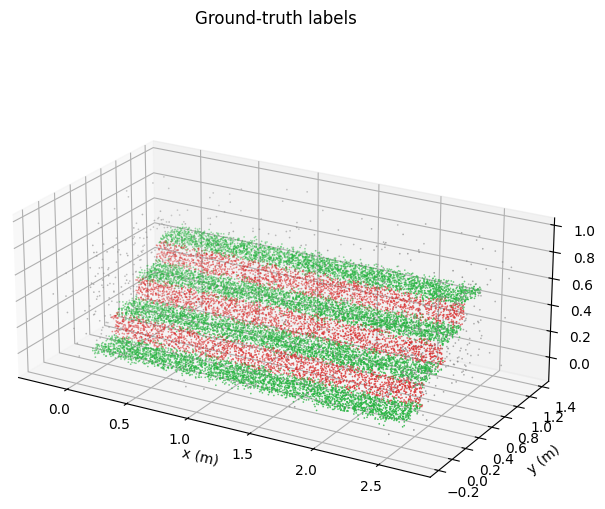
\includegraphics[width=0.95\linewidth]{raw_pointcloud.png}
\caption{Synthetic 4-step staircase point cloud, coloured by ground-truth label
(green: steppable tread, red: riser, grey: other). $\sim$18k points with LiDAR
noise and outliers.}
\label{fig:raw}
\end{figure}

\section{Methodology}
\label{sec:method}
All four methods output a per-point label in
$\{\textsc{steppable}, \textsc{riser}, \textsc{other}\}$. A surface is deemed
horizontal/vertical by the angle between its (unit) normal $\mathbf{n}$ and the
$z$-axis: with $n_z=|\mathbf{n}\cdot\hat{\mathbf z}|$, a surface is horizontal if
$n_z \ge \cos\theta_h$ and vertical if $n_z \le \cos\theta_v$, for thresholds
$\theta_h, \theta_v$.

\subsection{PCA Normal Analysis}
For each point we gather its $k$ nearest neighbours and form the local
covariance
\begin{equation}
C = \frac{1}{k}\sum_{j=1}^{k}(\mathbf{p}_j-\bar{\mathbf p})(\mathbf{p}_j-\bar{\mathbf p})^\top,
\end{equation}
Its eigenvector associated to the weakest eigenvalue estimates the surface normal
$\mathbf{n}$~\cite{rusu2011pcl}. Then points are directly classified by $n_z$.
This is the most local method and it is the most susceptible to surface jitter, but
it does not need a global model. We utilize $k=50$ neighbors, computed with the
nearest-neighbor search of scikit-learn~\cite{pedregosa2011scikit}.

\subsection{Multi-Plane RANSAC}
We iteratively fit planes using RANSAC~\cite{fischler1981ransac} and discard inliers
after each fit. The top edge of a riser is almost coplanar in $z$ with the tread
above it, so a na\"ive horizontal-first fitting leaks riser points into treads. We
thus first extract \emph{vertical} planes and then \emph{horizontal} planes with a
tight orientation tolerance ($\theta_h=15^\circ$, $\theta_v=75^\circ$) so that no
planes near the oblique staircase incline ($\approx31^\circ$) are permitted. A plane
is fitted from a minimal sample and scored by its number of inliers with a distance
criterion of $\tau=0.04$~m; planes with less than a minimum number of inliers are
rejected.

\subsection{Normal-Augmented DBSCAN with Slope Analysis}
Raw-$xyz$ DBSCAN~\cite{ester1996dbscan} collapses the whole staircase into one
connected component because adjacent treads and risers touch. We instead cluster
in the augmented feature space
\begin{equation}
\boldsymbol{\phi}(\mathbf{p}) = [\,x,\; y,\; z,\; w_n n_x,\; w_n n_y,\; w_n n_z\,],
\end{equation}
so two perpendicular but spatially near surfaces are separated by their different
normals. We utilize smoothed normals ($k=80$) and weight $w_n=2.0$. We use
$\varepsilon=0.20$ and \texttt{min\_samples}$=20$. Each resulting cluster is labeled
by the normal of its globally fitted plane. DBSCAN noise points become \emph{other}.

\subsection{Height-Histogram Tread Detection}
Treads are located in narrow, densely populated bands in $z$. We histogram $z$ with
1~cm precision, find local maxima above an adaptive prominence threshold, and mark
locations within a band of half-width $0.04$~m about each peak as potential treads,
refined by the local normal. This is a fast solution, and makes use of the
regularity of the staircase directly.

\section{Experimental Results}
\label{sec:results}
We evaluate the steppable class with Accuracy, Precision, Recall, F1, and IoU.
Precision and Recall are
$P=\frac{TP}{TP+FP}$, $R=\frac{TP}{TP+FN}$, with
$F1=\frac{2PR}{P+R}$ and $\text{IoU}=\frac{TP}{TP+FP+FN}$, where a positive is a
point predicted \textsc{steppable}. Table~\ref{tab:metrics} reports all methods
on the default cloud (seed fixed for reproducibility).

\begin{table}[t]
\centering
\renewcommand{\arraystretch}{1.1}
\caption{Steppable-class metrics on the default cloud (18{,}270 points).
Best per column in \textbf{bold}.}
\label{tab:metrics}
\begin{tabular}{lccccc}
\toprule
Method & Acc & P & R & F1 & IoU \\
\midrule
PCA normals       & \textbf{0.794} & 0.966 & \textbf{0.865} & \textbf{0.913} & \textbf{0.840} \\
Height-histogram  & 0.722 & 0.975 & 0.818 & 0.889 & 0.801 \\
DBSCAN + slope    & 0.769 & \textbf{0.977} & 0.796 & 0.877 & 0.782 \\
RANSAC multi-plane& 0.711 & 0.888 & 0.701 & 0.784 & 0.644 \\
\bottomrule
\end{tabular}
\end{table}

The PCA-normal approach has the best F1, IoU and best recall, whereas DBSCAN and
the height-histogram have the highest steppable precision ($\approx0.98$). The
before/after segmentation of the best technique is shown in Fig.~\ref{fig:seg} and
the confusion matrix is shown in Fig.~\ref{fig:cm}. The primary error mode is
steppable points being absorbed into \emph{other} near tread edges, rather than
confusion with risers.

\begin{figure*}[tp]
\centering
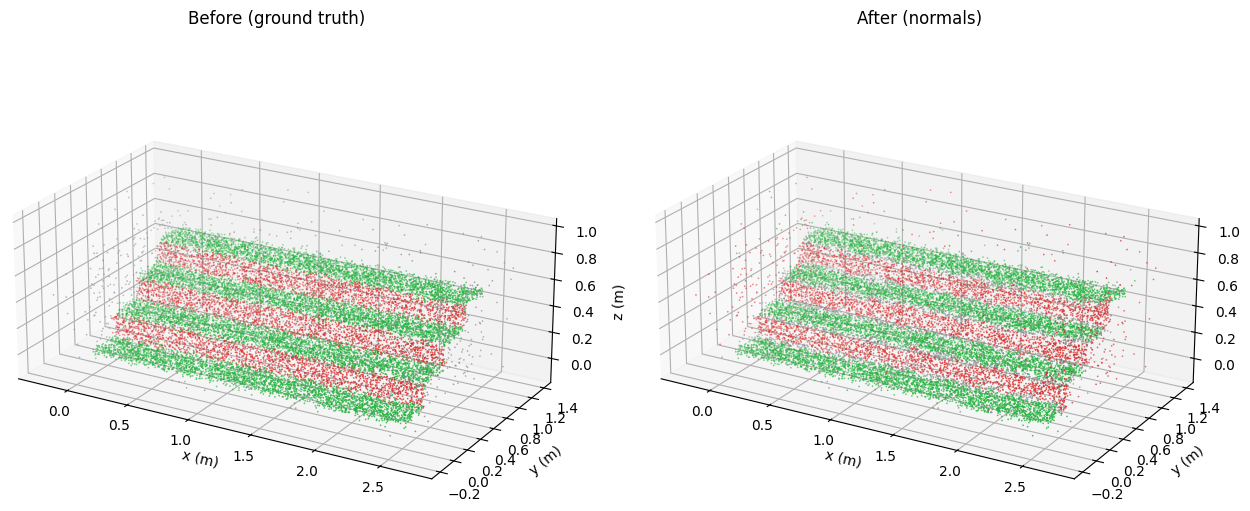
\includegraphics[width=0.82\textwidth]{before_after_normals.png}
\caption{Before/after segmentation by the PCA-normal method. Left: ground-truth
labels; right: predicted labels (green: steppable, red: riser, grey: other).}
\label{fig:seg}
\end{figure*}

\begin{figure}[t]
\centering
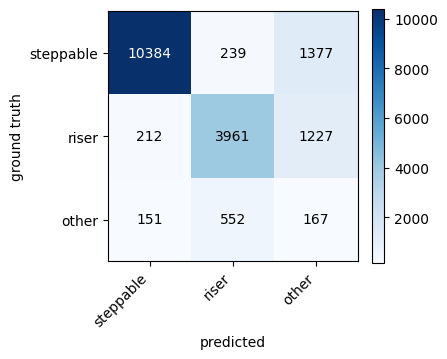
\includegraphics[width=0.62\linewidth]{confusion_normals.png}
\caption{Confusion matrix of the PCA-normal method; rows are ground truth, columns
predictions, ordered steppable / riser / other.}
\label{fig:cm}
\end{figure}

\subsection{Noise and Outlier Sensitivity}
We sweep the LiDAR noise $\sigma_L$ and outlier ratio $\rho$ and record the
steppable F1 (Fig.~\ref{fig:noise}). F1 drops from $0.918$ at $\sigma_L=0$ to
$0.861$ at $\sigma_L=0.02$ and $0.577$ at $\sigma_L=0.05$, showing local-normal
quality as the limiting factor: even the mandated per-step jitter
$\sigma_z=0.02$~m substantially reduces normals. Robustness to outliers is much
stronger: F1 only decreases from $0.918$ to $0.875$ when $\rho$ increases from $0$
to $0.20$, since outliers rarely form coherent planar support.

\begin{figure*}[tp]
\centering
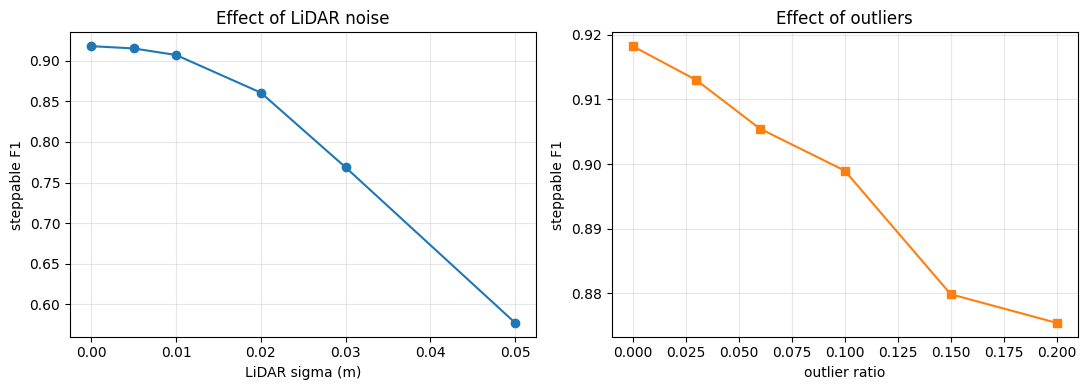
\includegraphics[width=0.74\textwidth]{noise_sensitivity.png}
\caption{Steppable F1 vs.\ LiDAR noise $\sigma_L$ (left) and outlier ratio
$\rho$ (right) for the PCA-normal method.}
\label{fig:noise}
\end{figure*}

\section{Analysis and Discussion}
\label{sec:discussion}
\textbf{Which metric matters for safety?} The cost of errors for a stair-following
robot is not symmetric. Dangerous is the step when tread is wanting; not to skip a
proper tread is not. Hence, the key objective is high \emph{precision} of the
steppable class, possibly at the expense of recall. The DBSCAN and height-histogram
approaches are attractive operating points under this criterion at $P\approx0.98$,
even though their F1 is below the PCA-normal method: a robot employing their output
would nearly never be directed to step on a non-tread.

\textbf{Local vs.\ global geometry.} The PCA-normal approach is fully local, and
hence inherits the full surface jitter. This is why the PCA-normal method has good
recall (it identifies virtually all genuine treads) but is sensitive to noise. The
plane- and cluster-based approaches are more cautious, more precise, since they
aggregate evidence over multiple sites.

\textbf{Is it safe enough?} A precision-driven approach results in very few
hazardous steppable calls for clean to moderate noise ($\sigma_L \le 0.02$~m),
which, when paired with a planner that selects only high-confidence, spatially
consistent footholds, forms a reasonable basis for a cautious controller. At high
noise ($\sigma_L\ge0.05$~m) both precision and recall drop and a single geometric
pass is no longer enough; temporal fusion across frames or a learnt refining stage
would be required.

\textbf{Limitations.} The data is generated and the staircase is regular and not
obstructed. Real scans introduce self occlusion, non-uniform density, specular
dropouts and clutter (e.g.\ railings, debris). The methods described here provide a
visible and reproducible baseline against which such impacts, including
learning-based methods, can be tested.

\section{Conclusion}
We provide a replicable comparison of four conventional geometric approaches for
the segmentation of steppable surfaces in a synthetic LiDAR staircase point cloud.
Overall, the PCA-normal technique performed the best (F1~$=0.913$, IoU~$=0.840$),
whereas normal-augmented DBSCAN and a height-histogram detector produced the highest
steppable precision ($\approx0.98$), which we claim is the deciding metric for
foothold safety. The noise analysis indicates that the binding restriction was
local-normal quality, not outliers. Future work involves evaluation on real scans,
temporal fusion and a hybrid that uses a high accuracy geometric prior to supervise
a learnt segmenter.

\FloatBarrier

\begin{thebibliography}{10}

\bibitem{kanoulas2018footstep}
D.~Kanoulas \emph{et al.}, ``Footstep planning in rough terrain for bipedal
robots using curved contact patches,'' in \emph{Proc. IEEE Int. Conf. Robotics
and Automation (ICRA)}, 2018, pp. 4662--4669.

\bibitem{nguyen2013segmentation}
A.~Nguyen and B.~Le, ``3D point cloud segmentation: A survey,'' in \emph{Proc.
IEEE Conf. Robotics, Automation and Mechatronics (RAM)}, 2013, pp. 225--230.

\bibitem{qi2017pointnet}
C.~R. Qi, H.~Su, K.~Mo, and L.~J. Guibas, ``PointNet: Deep learning on point sets
for 3D classification and segmentation,'' in \emph{Proc. IEEE Conf. Computer
Vision and Pattern Recognition (CVPR)}, 2017, pp. 652--660.

\bibitem{rusu2011pcl}
R.~B. Rusu and S.~Cousins, ``3D is here: Point Cloud Library (PCL),'' in
\emph{Proc. IEEE Int. Conf. Robotics and Automation (ICRA)}, 2011, pp. 1--4.

\bibitem{pedregosa2011scikit}
F.~Pedregosa \emph{et al.}, ``Scikit-learn: Machine learning in Python,''
\emph{Journal of Machine Learning Research}, vol. 12, pp. 2825--2830, 2011.

\bibitem{fischler1981ransac}
M.~A. Fischler and R.~C. Bolles, ``Random sample consensus: A paradigm for model
fitting with applications to image analysis and automated cartography,''
\emph{Communications of the ACM}, vol. 24, no. 6, pp. 381--395, 1981.

\bibitem{ester1996dbscan}
M.~Ester, H.-P. Kriegel, J.~Sander, and X.~Xu, ``A density-based algorithm for
discovering clusters in large spatial databases with noise,'' in \emph{Proc. 2nd
Int. Conf. Knowledge Discovery and Data Mining (KDD)}, 1996, pp. 226--231.

\bibitem{harris2020numpy}
C.~R. Harris \emph{et al.}, ``Array programming with NumPy,'' \emph{Nature}, vol.
585, pp. 357--362, 2020.

\bibitem{zhou2018open3d}
Q.-Y. Zhou, J.~Park, and V.~Koltun, ``Open3D: A modern library for 3D data
processing,'' \emph{arXiv preprint arXiv:1801.09847}, 2018.

\end{thebibliography}

\end{document}
